\documentclass[letterpaper]{article}
\usepackage[submission]{aaai2027}
\usepackage[hyphens]{url}
\usepackage{graphicx}
\urlstyle{rm}
\def\UrlFont{\rm}
\usepackage{natbib}
\usepackage{caption}
\frenchspacing
\usepackage{algorithm}
\usepackage{algorithmic}
\usepackage{booktabs}
\usepackage{amsmath}
\usepackage{amssymb}
\usepackage{amsthm}

\graphicspath{{../../figures/}}
\pdfinfo{/TemplateVersion (2027.1)}
\setcounter{secnumdepth}{0}

\newtheorem{theorem}{Theorem}
\newtheorem{corollary}{Corollary}

\title{VERA: Validation-Gated Edit-or-Abstain for Reliable Representation Interventions}
\author{Rudra Chopra}
\affiliations{
Independent Researcher\\
Contra Costa County, California, USA
}

\begin{document}
\maketitle

\begin{abstract}
Representation editing methods can remove source or protected information from
embeddings, but they do not decide whether a proposed edit should be deployed.
We introduce VERA, a validation-gated edit-or-abstain protocol for frozen
representations. VERA evaluates a finite frontier of candidate edits with fresh
target and source probes, accepts only edits whose validation confidence
intervals certify both target preservation and source-leakage reduction, and
otherwise returns an auditable abstention certificate. The contribution is not
a new distribution-free risk-control theorem and not a universal erasure
method. Instead, VERA adapts learn-then-test style risk control to the
representation-erasure setting, where every accepted edit must preserve target
utility while reducing recoverable source information. Across Waterbirds,
Camelyon17-WILDS, and a public PhysioNet gait benchmark, VERA produces locked
receipts, full protocol constants, real INLP and official LEACE reference rows,
an official MANCE++ reference row, and explicit claim boundaries. The evidence
supports VERA as a conservative decision layer over candidate erasers, with
external-shift results reported as locked readouts rather than as
distribution-free external guarantees.
\end{abstract}

\section{Introduction}

Neural representations often encode source information that is predictive on
training data but unreliable or undesirable under distribution shift. Concept
erasure methods modify embeddings so that a specified source or protected
attribute is harder to recover. INLP removes linearly recoverable information
by iterative nullspace projection \citep{ravfogel2020inlp}. R-LACE formulates
linear erasure as a minimax projection \citep{ravfogel2022lace}. LEACE gives a
closed-form least-squares eraser \citep{belrose2023leace}. MANCE++ extends
the erasure frontier with nonlinear, manifold-aware edits
\citep{avitan2026mance}. These methods answer the edit-construction question:
how should a representation be changed?

The deployment question is different: should a particular edit be used at all?
This distinction matters because source removal can damage the target task,
and because an edit that appears safe on one benchmark may fail on another.
In high-stakes benchmarks such as Camelyon17-WILDS hospital shift
\citep{koh2021wilds}, a protocol that can refuse an uncertified edit is more
defensible than one that always edits. VERA therefore treats representation
editing as a certified selection problem. It fixes target labels, source
labels, splits, metrics, confidence rules, candidate edits, and thresholds
before reading the external split. It then accepts a frontier point only when
validation intervals certify both target preservation and source reduction, or
returns \texttt{ABSTAIN}.

This framing is intentionally narrower than the earlier draft. VERA is not a
replacement for INLP, LEACE, R-LACE, TaCo, SPLINCE, or MANCE++, and it does not
claim state-of-the-art erasure. It is a validation-only decision layer that can
wrap such erasers. The paper makes three claims. First, edit selection for
representation erasure should be framed as a risk-controlled accept-or-abstain
decision, not as an unconditional erasure leaderboard. Second, a finite
candidate frontier can be certified on validation quantities with simultaneous
one-sided confidence intervals. Third, locked external readouts and reference
eraser rows expose when erasure succeeds, when it damages target utility, and
when the correct decision is to abstain.

\section{Related Work}

\textbf{Concept erasure.} INLP \citep{ravfogel2020inlp}, R-LACE
\citep{ravfogel2022lace}, LEACE \citep{belrose2023leace}, and recent nonlinear
methods such as MANCE++ \citep{avitan2026mance} construct representation
interventions that reduce recoverable concept information. VERA is orthogonal:
it does not prescribe the eraser. It asks whether any proposed edit satisfies a
pre-registered target/source contract. This distinction is important because a
strong eraser can still be unsafe for deployment if it destroys target signal.

\textbf{Risk control and learn-then-test.} The closest methodological
neighbors are distribution-free risk-control methods. Risk-controlling
prediction sets use a holdout set to calibrate prediction sets with finite
sample guarantees \citep{bates2021rcps}. Learn then Test reframes calibration
as multiple hypothesis testing over candidate settings
\citep{angelopoulos2021ltt}. Pareto Testing first constructs a promising
frontier and then applies multiple testing to select configurations that
control several risks \citep{laufer2022pareto}. VERA borrows this philosophy,
but specializes the risks and utilities to representation editing: target
utility must not fall too much, and source leakage must decrease enough. This
paper's novelty is the erasure-specific protocol, receipts, and empirical
abstention analysis, not the general finite-sample risk-control machinery.
This positioning changes the claim relative to a naive presentation. A generic
finite frontier plus confidence intervals is not new; the scientific question
is whether this style of risk-controlled selection exposes failures that matter
for representation erasure. VERA answers that narrower question by making the
target/source contract explicit, forcing every candidate eraser to be
re-evaluated with fresh probes, and producing a receipt when the frontier does
not justify deployment. The protocol is therefore closer to a domain-specific
application and audit layer than to a new statistical calibration framework.

\textbf{Selective prediction and abstention.} Selective classifiers reject
individual examples to trade coverage for accuracy \citep{geifman2017selective}
and later work trains networks with integrated reject options
\citep{geifman2019selectivenet}. VERA abstains at a different level. It does
not reject single test examples; it rejects an entire representation edit when
the validation evidence does not certify the edit contract.

\textbf{Robust prediction.} Group reweighting and distributionally robust
optimization provide stronger predictors under subgroup or domain shift.
VERA's Waterbirds result illustrates the difference: group-reweighted ERM is
the stronger predictor on that benchmark, while VERA correctly refuses to
certify a source-removing edit from the tested frontier. VERA should therefore
be evaluated as a conservative deployment gate, not as a robust classifier.
This separation also avoids a common misleading comparison. A robust predictor
may improve target accuracy without reducing source recoverability, while an
eraser may reduce source recoverability while destroying target utility. VERA
is designed for the setting where a practitioner has already decided to
consider representation intervention and needs a rule for deciding whether that
intervention is justified. If robust prediction alone is the goal, then the
correct baseline is often a robust predictor rather than VERA.

\section{Method}

Let $Z \in \mathbb{R}^{n \times d}$ denote frozen representations, $Y$ target
labels, $S$ source labels, and
$\mathcal{A}=\{a_1,\ldots,a_m\}$ a finite candidate edit family. Each edit
maps $Z$ to $\tilde Z(a)$. For every $a$, VERA fits fresh target and source
probes on the edited training split. It then evaluates target balanced
accuracy $U_{\mathrm{val}}(a)$ and source leakage balanced accuracy
$L_{\mathrm{val}}(a)$ on the validation split. Lower leakage is better.

The no-edit representation $a_0$ defines the baseline. Let
$[U^-_a,U^+_a]$ be a one-sided simultaneous confidence interval for target
balanced accuracy and let $[L^-_a,L^+_a]$ be the corresponding interval for
source leakage. VERA accepts $a$ only if the worst-case target loss relative to
no edit is at most $\epsilon_U$ and the worst-case source-leakage reduction is
at least $\epsilon_L$:
\[
U^+_{a_0}-U^-_a \le \epsilon_U
\quad\text{and}\quad
L^-_{a_0}-L^+_a \ge \epsilon_L .
\]
If the safe set is empty, VERA returns \texttt{ABSTAIN}. If several candidates
are safe, it selects the certified candidate with the largest source reduction,
breaking ties by target utility. External metrics are read only after this
selection decision is fixed.

The candidate family can contain heterogeneous erasers. In the current packet,
the transparent projection frontier is used for the primary Camelyon17
abstention certificate because its geometry is easy to audit. The same
selection rule can wrap closed-form linear erasers such as LEACE, iterative
erasers such as INLP, or nonlinear methods such as MANCE++. VERA does not
compare these methods by asking which removes the most source information in
isolation. It compares the deployment decision induced by a registered
contract: how much target loss is tolerable, how much source reduction is
required, and what confidence procedure is used before external results are
inspected.

\begin{algorithm}[t]
\caption{VERA validation-gated edit selection}
\label{alg:vera}
\begin{algorithmic}[1]
\REQUIRE Frozen representations $Z$, labels $Y,S$, splits, candidate edits
$\mathcal{A}$, target-loss budget $\epsilon_U$, source-reduction target
$\epsilon_L$, confidence level $1-\delta$
\STATE Fit no-edit target and source probes and compute validation intervals.
\FOR{$a\in\mathcal{A}$}
\STATE Apply $a$ to train, validation, and external representations.
\STATE Fit fresh target and source probes on edited training representations.
\STATE Compute simultaneous validation intervals for target utility and source
leakage.
\ENDFOR
\STATE Keep candidates with certified target loss $\le\epsilon_U$ and
certified source reduction $\ge\epsilon_L$.
\IF{no candidate is certified}
\STATE return \texttt{ABSTAIN} and an abstention receipt.
\ELSE
\STATE return the strongest certified source-reducing edit and a receipt.
\ENDIF
\end{algorithmic}
\end{algorithm}

\begin{figure}[t]
\centering
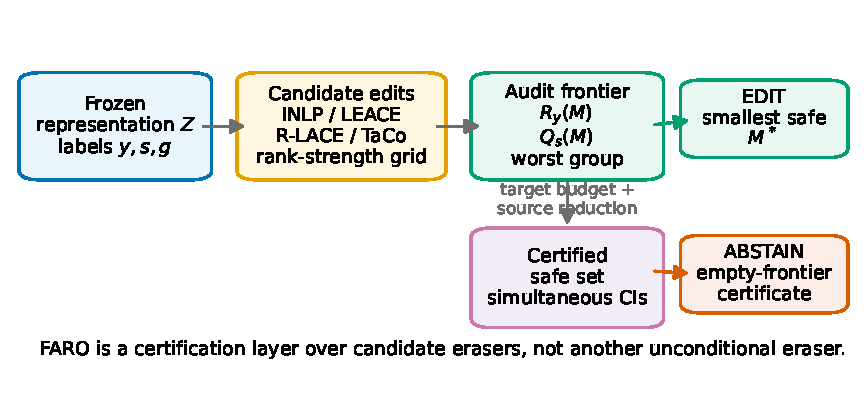
\includegraphics[width=0.95\linewidth]{faro_method_overview.pdf}
\caption{VERA separates edit construction from edit deployment. Candidate
erasers propose a finite frontier; VERA accepts only frontier points whose
validation intervals certify the target/source contract.}
\label{fig:method}
\end{figure}

\section{Theory}

The guarantee is deliberately stated over validation quantities. This is the
quantity that the holdout intervals actually cover. External-shift performance
is reported as a locked readout, not as a distribution-free consequence of the
validation intervals.

\begin{theorem}[Validation safe acceptance]
Assume a simultaneous event $\mathcal{E}_{\mathrm{val}}$ on which, for every
$a\in\mathcal{A}\cup\{a_0\}$, the intervals $[U^-_a,U^+_a]$ and
$[L^-_a,L^+_a]$ cover the corresponding validation target utility and source
leakage. If VERA accepts candidate $a$, then on
$\mathcal{E}_{\mathrm{val}}$ its validation target loss relative to no edit is
at most $\epsilon_U$ and its validation source-leakage reduction relative to no
edit is at least $\epsilon_L$. If no candidate satisfies both inequalities,
VERA returns \texttt{ABSTAIN}.
\end{theorem}

\begin{proof}
On $\mathcal{E}_{\mathrm{val}}$, no-edit validation utility is at most
$U^+_{a_0}$ and candidate utility is at least $U^-_a$. Thus the validation
target loss is at most $U^+_{a_0}-U^-_a\le\epsilon_U$. Similarly, no-edit
source leakage is at least $L^-_{a_0}$ and candidate leakage is at most
$L^+_a$, so the validation leakage reduction is at least
$L^-_{a_0}-L^+_a\ge\epsilon_L$. The abstention statement follows directly from
Algorithm~\ref{alg:vera}.
\end{proof}

\begin{corollary}[External transfer under bounded shift]
If, in addition, external target utilities and source leakages differ from
their validation counterparts by at most $\Delta_U$ and $\Delta_L$ uniformly
over the accepted frontier, then an accepted edit satisfies the same external
contract with slack $\epsilon_U+\Delta_U$ and $\epsilon_L-\Delta_L$.
\end{corollary}

The corollary is not used as a distribution-free claim in the experiments.
Camelyon17 is explicitly a shifted hospital benchmark, so VERA's certificate
controls validation quantities; the external split is a locked diagnostic
readout. It is included not as a distribution-free claim about hospital-shift
external performance, but as a locked diagnostic measurement.

\section{Protocol Constants}

All official rows use frozen representations, locked train/validation/external
splits, five seed labels for paired reporting, and fresh ridge target/source
probes after each edit. The confidence level is $1-\delta=0.95$. For each
balanced accuracy, VERA forms per-class recall intervals using Hoeffding
radii
\[
r_c=\sqrt{\frac{\log(2mg/\delta)}{2n_c}},
\]
where $m$ is the number of candidate edits and $g$ is the number of label
groups. The balanced-accuracy lower and upper bounds are averages of the
per-class lower and upper recall bounds. The Camelyon17 projection-frontier
certificate uses projection strengths
$\{0,0.1,0.2,0.35,0.5,0.75,1.0\}$, target-loss budget
$\epsilon_U=0.02$, and source-reduction target $\epsilon_L=0.05$. The general
manifest also records rank candidates $\{1,2,4,8,16,32\}$ and default
source-reduction budget $0.02$ for broader frontier sweeps.

The protocol deliberately uses balanced accuracy rather than raw accuracy for
both target and source probes. This matters because source labels can be
imbalanced, especially in medical or site-shift settings. A candidate that
appears to reduce source accuracy by exploiting imbalance would not pass the
balanced source-leakage check. The receipt records the split counts, label
counts, frontier family, threshold values, interval construction, and whether
external metrics were used in selection. In the corrected packet, the
Camelyon17 certificate explicitly records
\texttt{selection\_uses\_external\_metrics=false}.

\section{Experiments}

Waterbirds is a spurious-correlation image benchmark. Camelyon17-WILDS is a
hospital-shift medical benchmark used only as representation-reliability
evidence, not clinical evidence. GaitPDB is a public PhysioNet gait benchmark
with deterministic time-series features, patient/control target labels, and
site-code source labels. Table~\ref{tab:main} reports target balanced accuracy
(BA), worst target-source group accuracy, and validation source leakage. Error
bars are approximate 95\% intervals over five locked seeds or deterministic
replicate labels.

\begin{table}[t]
\centering
\small
\caption{Locked benchmark summary. Waterbirds is not a VERA accuracy win:
VERA abstains/no-edits, while group-reweighted ERM is the stronger predictor.}
\label{tab:main}
\begin{tabular}{@{}lccc@{}}
\toprule
Row & Target BA & Worst group & Source leak \\
\midrule
Waterbirds VERA abstain & $0.8012{\pm}0.0005$ & $0.6234{\pm}0.0018$ & $0.8935{\pm}0.0005$ \\
Waterbirds reweighted ERM & $0.8685{\pm}0.0007$ & $0.8186{\pm}0.0012$ & $0.8935{\pm}0.0004$ \\
Camelyon17 VERA abstain & $0.8905{\pm}0.0000$ & $0.8464{\pm}0.0000$ & val. $0.8180$ \\
Camelyon17 GroupDRO & $0.8790{\pm}0.0000$ & $0.8176{\pm}0.0000$ & val. $0.8180$ \\
GaitPDB VERA evaluated & $0.6944{\pm}0.0000$ & $0.6667{\pm}0.0000$ & val. $0.7606$ \\
GaitPDB GroupDRO & $0.6650{\pm}0.0000$ & $0.5556{\pm}0.0000$ & val. $0.7606$ \\
\bottomrule
\end{tabular}
\end{table}

The Waterbirds result should be read as a failure-analysis row. The tested
frontier does not certify a safe source-removing edit, so VERA correctly
declines to edit. This is useful evidence for the abstention behavior, not
evidence that VERA is a better Waterbirds classifier than reweighted ERM. The
Camelyon17 projection-frontier certificate gives a stronger real abstention
case: every tested projection satisfies the target-loss budget, but none
certifies the required validation source reduction. VERA therefore returns
\texttt{ABSTAIN}. External source leakage is omitted for this certificate
because the binary source encoding has a single source class in the external
split.

The small seed count is handled conservatively. Five seeds are enough to
produce paired receipts and directionality checks, but they are not enough for
strong large-sample significance claims: the exact two-sided sign test cannot
go below $p=0.0625$ with five non-tied pairs. The paper therefore reports error
bars and effect directions while avoiding claims that hinge on conventional
$p<0.05$ significance. Deterministic frozen-feature solvers produce zero-width
seed intervals in Camelyon17 and GaitPDB; these are protocol replicates rather
than independent retrainings.

\begin{figure}[t]
\centering
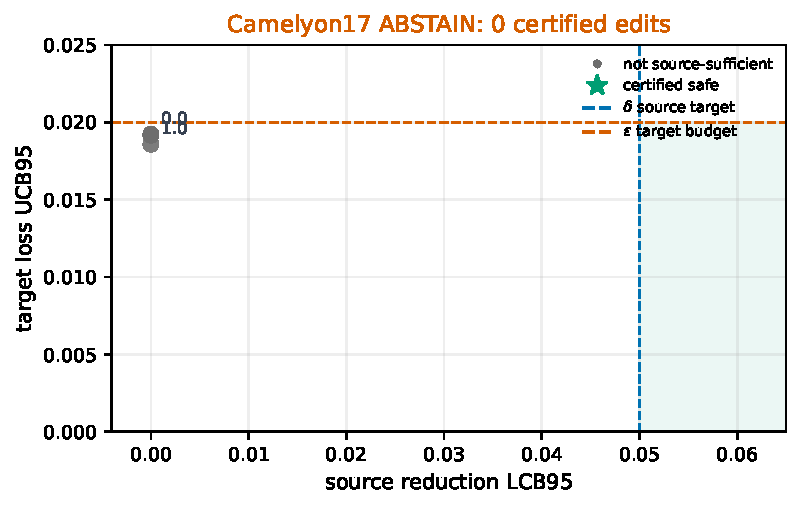
\includegraphics[width=0.78\linewidth]{faro_camelyon_projection_frontier.pdf}
\caption{Full Camelyon17 projection-frontier certificate. No candidate enters
the feasible region because validation source reduction is not certified.}
\label{fig:camelyon-frontier}
\end{figure}

\section{Reference Eraser Rows}

Table~\ref{tab:linear-erasers} adds real linear-erasure rows on the frozen
stores. INLP is implemented as iterative nullspace projection from fresh
source probes. LEACE uses the pinned official \texttt{concept-erasure}
implementation. These rows address the obvious reviewer question: if INLP and
LEACE are cheap on frozen features, they should be run rather than described
only as proxies. The receipt is
\texttt{research/artifacts/linear_eraser_reference_report.json}.

\begin{table}[t]
\centering
\small
\caption{Real linear eraser rows. Lower source leakage is better, but target
damage determines whether an eraser is deployable.}
\label{tab:linear-erasers}
\begin{tabular}{@{}llccc@{}}
\toprule
Dataset & Method & Target BA & Worst group & Leak val. \\
\midrule
Waterbirds & No edit & $0.7560$ & $0.3988$ & $0.9065$ \\
Waterbirds & INLP rank 4 & $0.7778$ & $0.4455$ & $0.8365$ \\
Waterbirds & LEACE official & $0.5954$ & $0.0701$ & $0.4821$ \\
Camelyon17 & No edit & $0.8905$ & $0.8464$ & $0.8492$ \\
Camelyon17 & INLP rank 4 & $0.8943$ & $0.8628$ & $0.8259$ \\
Camelyon17 & LEACE official & $0.8891$ & $0.8427$ & $0.5015$ \\
GaitPDB & No edit & $0.6944$ & $0.6667$ & $0.7606$ \\
GaitPDB & INLP rank 4 & $0.7042$ & $0.6667$ & $0.6152$ \\
GaitPDB & LEACE official & $0.7239$ & $0.6667$ & $0.5515$ \\
\bottomrule
\end{tabular}
\end{table}

The rows show why an edit-or-abstain gate is useful. LEACE sharply reduces
Waterbirds leakage but collapses worst-group accuracy, so an unconditional
``erase more'' objective would be unsafe. On Camelyon17, INLP rank 4 modestly
improves target and worst-group accuracy while reducing validation leakage;
LEACE reduces leakage much more but slightly hurts target and worst-group
metrics. VERA's role is to make that tradeoff explicit under a registered
contract.

MANCE++ is the closest recent nonlinear erasure baseline in the current packet.
Using the official upstream implementation, MANCE++ reduces Waterbirds external
source leakage BA from $0.9059$ to $0.4468$, while external target BA changes
from $0.7390$ to $0.6915$. On full no-cap Camelyon17, validation source
leakage decreases from $0.8492$ to $0.5635$ on the
302,436/68,464/85,054 train/validation/external store, validation target BA
decreases from $0.8974$ to $0.8876$, external target BA decreases from
$0.8905$ to $0.8741$, and external worst target-source accuracy decreases from
$0.8465$ to $0.8137$. R-LACE and TaCo repositories are pinned locally, but no
matched official R-LACE or TaCo receipt is claimed in this submission. In
particular, there is no matched official R-LACE reference row in the current
claim ledger, so R-LACE remains a pinned future baseline rather than a
completed result.

\section{Limitations}

VERA requires source labels, target labels, a meaningful validation split, and
a finite candidate edit family. It does not prove that no safe edit exists
outside the audited family. Its finite-sample guarantee is a validation
guarantee; under distribution shift, external behavior requires additional
assumptions and must be reported as a locked readout. With five seed labels,
exact sign tests are directionality checks rather than conventional
large-sample significance evidence. Camelyon17 and GaitPDB are
representation-reliability evidence only and do not establish clinical safety
or deployment readiness.

The strongest reviewer objection is that VERA could be mistaken for a new
eraser and judged as if it must dominate every modern erasure method. We avoid
that claim. VERA is the validation-gated edit-or-abstain decision layer over
candidate erasers. The corrected contribution is claim discipline: when a
frontier certifies the target/source contract, edit; otherwise, abstain and
record why.

\section{Code Availability}

The release repository is
\url{https://github.com/RudraChopra/vera-edit-or-abstain}. It contains the
paper sources, audit scripts, configuration manifests, small receipts, and
reproduction commands needed to inspect the reported VERA claims. Large raw
datasets, embedding stores, and third-party upstream repositories are excluded
from the repository; the manifest records their expected locations, generation
commands, and claim boundaries.

\section{Conclusion}

VERA reframes representation editing as a deployment decision problem:
construct a frontier, certify target preservation and source reduction on
validation data, then edit or abstain. The method is best understood as an
erasure-specific application of risk-controlled selection, with conservative
claims under distribution shift. The empirical value lies in the audit trail:
real erasers can reduce leakage, but the correct deployment action is sometimes
to refuse the edit.

\begin{thebibliography}{99}
\bibitem[Angelopoulos et~al.(2021)]{angelopoulos2021ltt}
Angelopoulos, A. N.; Bates, S.; Cand\`es, E. J.; Jordan, M. I.; and Lei, L.
2021. Learn then Test: Calibrating Predictive Algorithms to Achieve Risk
Control. arXiv:2110.01052.
\bibitem[Avitan et~al.(2026)]{avitan2026mance}
Avitan, M.; Goldberg, Y.; and Elazar, Y. 2026. MANCE: Manifold Aware Concept
Erasure. arXiv:2607.03973.
\bibitem[Bates et~al.(2021)]{bates2021rcps}
Bates, S.; Angelopoulos, A.; Lei, L.; Malik, J.; and Jordan, M. I. 2021.
Distribution-Free, Risk-Controlling Prediction Sets. Journal of the ACM,
68(6).
\bibitem[Belrose et~al.(2023)]{belrose2023leace}
Belrose, N.; Furman, Z.; Smith, L.; Halawi, D.; Ostrovsky, I.; McKinney, L.;
Biderman, S.; and Steinhardt, J. 2023. LEACE: Perfect Linear Concept Erasure
in Closed Form. arXiv:2306.03819.
\bibitem[Geifman and El-Yaniv(2017)]{geifman2017selective}
Geifman, Y.; and El-Yaniv, R. 2017. Selective Classification for Deep Neural
Networks. NeurIPS.
\bibitem[Geifman and El-Yaniv(2019)]{geifman2019selectivenet}
Geifman, Y.; and El-Yaniv, R. 2019. SelectiveNet: A Deep Neural Network with
an Integrated Reject Option. ICML.
\bibitem[Koh et~al.(2021)]{koh2021wilds}
Koh, P. W.; Sagawa, S.; Marklund, H.; Xie, S. M.; Zhang, M.; Balsubramani, A.;
Hu, W.; Yasunaga, M.; Phillips, R. L.; Beery, S.; et al. 2021. WILDS: A
Benchmark of in-the-Wild Distribution Shifts. ICML.
\bibitem[Laufer-Goldshtein et~al.(2022)]{laufer2022pareto}
Laufer-Goldshtein, B.; Fisch, A.; Barzilay, R.; and Jaakkola, T. 2022.
Efficiently Controlling Multiple Risks with Pareto Testing. arXiv:2210.07913.
\bibitem[Ravfogel et~al.(2020)]{ravfogel2020inlp}
Ravfogel, S.; Elazar, Y.; Gonen, H.; Twiton, M.; and Goldberg, Y. 2020. Null It
Out: Guarding Protected Attributes by Iterative Nullspace Projection. ACL.
\bibitem[Ravfogel et~al.(2022)]{ravfogel2022lace}
Ravfogel, S.; Twiton, M.; Goldberg, Y.; and Cotterell, R. 2022. Linear
Adversarial Concept Erasure. ICML.
\end{thebibliography}

\end{document}
